\subsection{Definition of Procedures}
A procedure in the FW Profile consists of the following elements:

\begin{fw_itemize}
\item One \emph{initial node}
\item One or more \emph{actions nodes} (or actions)
\item One or more \emph{control flows}
\item Zero or more \emph{decision nodes}
\item Zero or more \emph{final nodes}
\item Two \emph{execution counters}
\end{fw_itemize}

The \emph{initial node} is characterized by one control flow which has the initial node as its source
and has either an action node or a decision node as its target.

An \emph{action node} (or action) is characterized by the following elements:

\begin{fw_itemize}
\item One or more incoming control flows
\item One outgoing control flow
\item The behaviour associated to the action
\end{fw_itemize}

The incoming control flows are control flows which have the action as its target. The outgoing
control flow is a control flow which has the action as its source.

An action represents a single step within a procedure. It encapsulates behaviour that is not
decomposed further within the procedure. The action's behaviour can be defined using natural
language or some formalism (e.g. an \"action language\").

A \emph{control flow} is characterized by the following elements:

\begin{fw_itemize}
\item One source
\item One target (or destination)
\item Zero or one guards
\end{fw_itemize}

The source and the target are either action nodes or decision nodes. Additionally, the initial
node can be the source of a control flow and the final node can be the destination of one or
more control flows.

The guard is a specification which evaluates either to TRUE or FALSE and which
has no side effects. Absence of a guard is equivalent to a guard which always evaluates to TRUE.

A \emph{decision node} is characterized by the following elements:
\begin{fw_itemize}
\item One or more \emph{incoming control flows}
\item Two or more \emph{outgoing control flows}
\end{fw_itemize}

The incoming control flows are control flows that have the decision node as its target. The
outgoing control flow are control flows that have the decision node as their source.

For control flows issuing from a decision node, the pre-defined \textit{Else} guard is available. This
guard returns TRUE if and only if all the other guards attached to control flows issuing from
the same decision node return FALSE.

The \emph{final node} is characterized by one or more incoming control flows (namely control flows
that have the final node as their target). Note that all final nodes are equivalent and therefore it
would be legitimate to allow only one single final node. The option to have more than one is
introduced as a matter of convenience.

The \emph{execution counters} are unsigned integers which are exclusively characterized by their value.
The first execution counter is called the \emph{Procedure Execution Counter} and the second one
is called the \emph{Node Execution Counter}.

The following syntactical constraints apply to the definition of the procedure elements:

\begin{fw_itemize}
\item C1. The control flows out of a decision node must have a guard.
\end{fw_itemize}

The following dynamical constraints must be satisfied when a procedure is executed:
\begin{fw_itemize}
\item D1. Among the outgoing control flows from a decision node, at least one must have a
guard which evaluates to true;
\item D2. The evaluation of the guards of a control flow must be free of side-effects;
\item D3. The procedure actions and guards must execute in zero logical execution time
(i.e. on an infinitely fast processor and in the absence of pre-emption or blocking, 
they must execute in zero time).
\end{fw_itemize}

The last constraint implies that the behaviour encapsulated by the actions and by the guards
must be purely functional. In practice, this means that actions and guards cannot include time-
dependent behaviour or behaviour that depends on synchronization with other flows of
executions.

The execution counters of a procedure count the number of times the procedure has
been executed (one counts the number of times the procedure has been executed since it 
was started and the other counts the number of times the procedure has been executed
since its current node was entered). Since procedures will often be executed periodically,
the execution counters can serve as proxies for measuring the elapsing of time.


\subsection{Procedure Behaviour}\label{sec:procBehaviour} 
Four operations may be performed on a procedure: (a) the procedure may be \emph{started}; (b) the
procedure may be \emph{executed}; (c) the procedure may be \emph{stopped}; or (d) the procedure may be
\emph{run}.

Procedures are purely reactive: they wait for one of these four operations to be performed upon
them and they only execute a behaviour in response to one of these operations.

Operations are performed in response to \emph{commands}: the command Start triggers the start
operation; the command Execute triggers the execute operation; the command Stop triggers the
stop operation; and the command Run triggers the run operation.

A procedure may be in two states: STOPPED or STARTED. Initially, by default, the procedure
is in state STOPPED. When the procedure is in state STARTED, it has a \emph{current node}. The
current node is either the procedure's initial node or one of its action nodes.

When a procedure is \emph{started}, the following behaviour is executed:
\begin{fw_enumerate}
\item If the procedure is in state STARTED, then no further action is performed;
\item If the procedure is in state STOPPED, then it is put in state STARTED, its current
node is set equal to its initial node and its execution counters are reset.
\end{fw_enumerate}

When a procedure is \emph{stopped}, the following behaviour is executed:

\begin{fw_enumerate}
\item If the procedure is in state STOPPED, then no further action is performed;
\item If the procedure is in state STARTED, then it is put in state STOPPED and its current
node is set to an invalid value.
\end{fw_enumerate}

Thus, the Stop and Start commands toggle the state of a procedure and update its current node.
This is shown in the state diagram of figure \ref{fig:PR_StartStop}.

\begin{figure}[ht]
 \centering
 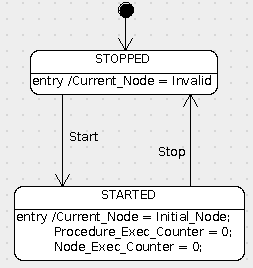
\includegraphics[scale=0.5,keepaspectratio=true]{PR_StartStop.png}
 \caption{Procedure Start/Stop Commands}
 \label{fig:PR_StartStop}
\end{figure}

When a procedure is \emph{executed}, the following behaviour is executed:
\begin{fw_enumerate}
\item If the procedure is in state STOPPED, then no further action is performed;
\item If the procedure is in state STARTED, then its execution counters are incremented
by 1 and the guard attached to the outgoing control flow of the current node is evaluated;
\item If the guard evaluates to FALSE, then no further action is performed;
\item If the guard evaluates to TRUE and the target of the outgoing control flow attached to
the current node is an action node T, then: (a) the current node is set equal to T, (b) the
node execution counter is reset, (c) the
behaviour associated to T is executed, (d) the guard on the out-going control flow of T is evaluated
and steps 3 and 4 are (recusively) repeated;
\item If the guard evaluates to TRUE and the target of the outgoing control flow attached to
the current node is a decision node, then: (a) the guards of the outgoing control flows
attached to the decision node are evaluated; (b) if the target of the outgoing control
flow whose guard evaluates to TRUE is another decision node, then steps (a) to (d) are
performed upon it; (c) if the target of the outgoing control flow whose guard evaluates
to TRUE is an action node T, then the current node is set equal to T, the behaviour
associated to T is executed, the guard on the out-going control flow of T is evaluated
and steps 3 and 4 are (recusively) repeated; (d) if the target of the
outgoing control flow whose guard evaluates to TRUE is a final node, the state of the
procedure is set to STOPPED and the current node is set equal to an invalid value.
\item If the guard evaluates to TRUE and the target of the outgoing control flow attached to
the current node is a final node, then the state of the procedure is set to STOPPED,
and the current node is set equal to an invalid value.
\end{fw_enumerate}

Thus, in summary, when a procedure is executed, it tries to traverse the control flow issuing
form the current node. If this can be done (i.e. if the guard associated to the control flow
evaluates to true), then it advances the execution of the procedure until it finds a guard that
evaluates to false or until it finds a final node. Whenever an action node is traversed, its
associated behaviour is executed.

The Execute command may carry parameters. These parameters may be passed to any of the
actions that are executed as part of the processing of the Execute command.

Note that, at any given time, only one flow of control may be traversing a procedure. This flow
of control is advanced every time that the procedure is executed.

The behaviour associated to the execution of a procedure is shown as an activity diagram in
figure \ref{fig:PR_Execution}.

Finally, when a procedure is run, the following behaviour is executed:

\begin{fw_enumerate}
\item The procedure is started;
\item The procedure is executed;
\item The procedure is stopped. 
\end{fw_enumerate}

Thus, the Run operation is defined in terms of the previous three operations. The Run
operation may take parameters which are passed to the Execute operation which is performed
as part of the Run operation (step 2 above).

The Run operation is only useful for procedures which execute in one single cycle. It is
typically used to perform the actions associated to a state in a state machine.

The execution of the various actions associated to the four procedure operations (Start,
Execute, Stop, and Run) is performed in sequence: an action is executed only when the
previous one has completed. Note that, since actions are constrained to execute in zero logical
time, the execution of a procedure operation will also execute in zero logical time.

Requests to perform an operation upon a procedure are executed in sequence. A new request
can only be processed by a procedure when the previous one has been fully processed.
Procedures have no queues to buffer incoming operation requests.

Note that the procedure operations do not return any values.

\begin{figure}[ht]
 \centering
 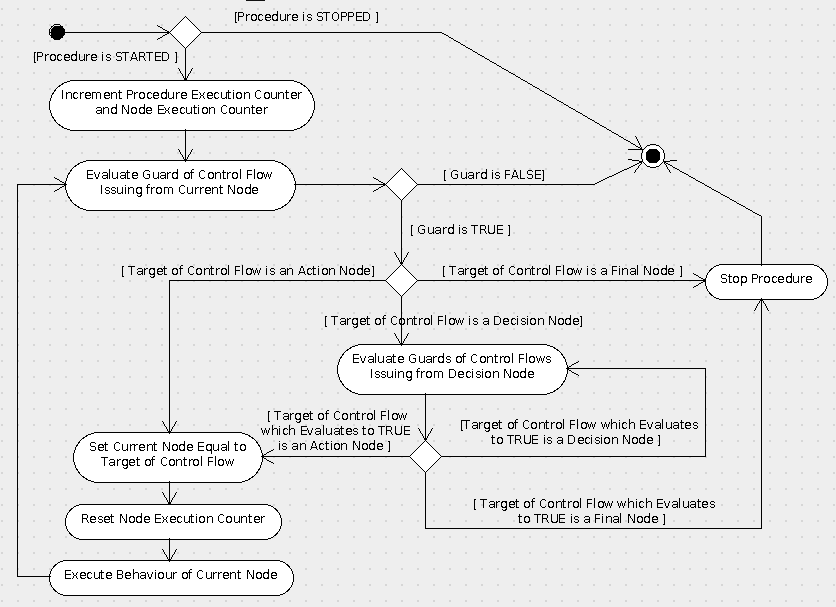
\includegraphics[scale=0.4,keepaspectratio=true]{PR_Execution.png}
 \caption{Procedure Execution Logic}
 \label{fig:PR_Execution}
\end{figure}

\subsection{UML 2 Compliance}
The procedure model offered by the FW Profile complies with the UML 2 activity model in
the sense that the elements of the procedure concept of the FW Profile and their semantics can
be mapped in an obvious way to a subset of the elements of the activity concept of UML 2.

The execution counters are specific to the FW Profile. They have been introduced as a
substitute for the concept of time (which does not exist in the FW Profile Procedures) in
the sense that, if procedures are executed periodically, then the value of their execution 
counters is proportional to the time elapsed since the procedure was started (Procedure
Execution Counter) or since the current node was entered (Node Execution Counter). 

